\documentclass{standalone}
\usepackage{tikz}

\begin{document}
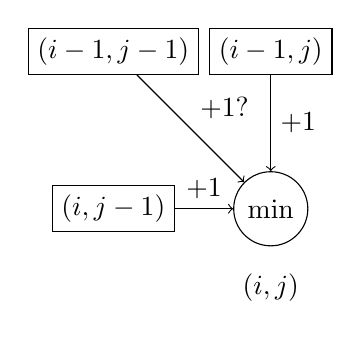
\begin{tikzpicture}[scale=2]
\node[draw] (imjm) at (-1, 1) {$(i - 1, j - 1)$};
\node[draw] (ijm) at (-1, 0) {$(i, j - 1)$};
\node[draw] (imj) at (0, 1) {$(i - 1, j)$};
\node[circle,draw] (ij) at (0, 0) {min};
\node[below of=ij] {$(i, j)$};
\draw[->] (imjm) edge node[above right] {+1?} (ij);
\draw[->] (imj) edge node[right] {+1} (ij);
\draw[->] (ijm) edge node[above] {+1} (ij);
\end{tikzpicture}
\end{document}